\subsubsection{Différences}
	\begin{itemize}
		\item Réalisation d'une requête PUT via l'api REST.
		\item Amélioration de l'aspect graphique. 
		\item Utilisation du \textit{SecurityAuthenticator} du backend pour ajouter l'utilisateur dans le système.
		\item Ajout de l'inscription automatique de l'utilisateur au séance (voir \ref{Inscription auto} ). 
	\end{itemize}


\subsubsection{Diagramme de séquence}
	\begin{figure}[h]
		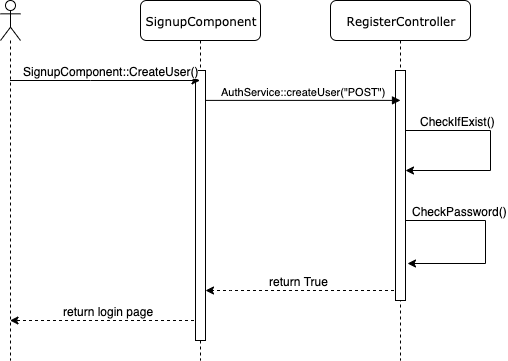
\includegraphics[width=\textwidth,center]{Diagramme/sequence-us1-angular}
		\caption{Diagramme de séquence de l'inscription d'un utilisateur. }
	\end{figure}
	
\newpage
\subsubsection{Scripts concernés}
	\begin{itemize}
		\item \Href{https://github.com/victorsmits/Aquabike/blob/master/frontend/src/app/service/auth.service.ts}{auth.service.ts}
		\item \Href{https://github.com/victorsmits/Aquabike/blob/master/backend/src/Controller/API/SecurityControllerAPI.php}{SecurityControllerAPI.php}
		\item \Href{https://github.com/victorsmits/Aquabike/blob/master/backend/src/Entity/Person.php}{Person.php}
		\item \Href{https://github.com/victorsmits/Aquabike/blob/master/frontend/src/app/signup/signup.component.ts}{signup.component.ts}
		\item \Href{https://github.com/victorsmits/Aquabike/blob/master/frontend/src/app/signup/signup.component.html}{signup.component.html}
	\end{itemize}